
\documentclass{report}
\usepackage[ansinew]{inputenc}
\usepackage[french]{babel}
\usepackage{amsmath}
\usepackage{graphicx}
%\usepackage{psfig}
\include{epsf}
%\textwidth 19cm
%\textheight 25cm
%\leftmargin -2cm


\begin{document}

\title{Madvertise: ML task}
\author{Wuilloud Jair}
\date{$14.05.2013$}
\maketitle




\pagebreak

\paragraph{My Understanding and Decomposition of the Problem}

\subparagraph{ Basic Idea: }
"Bayesian statistics indicates us how to adapt our belief when acquiring when acquiring new data".
I start recalling Baye's first law:
$$
p(Clicked | Data) = \frac{p(Data | Clicked)p(Clicked)}{p(Data)},
$$
In our context, $Data$ means some parameter configuration. 
The problems are then to select out a parameter subset for which the 
above formula could be adapted and compute the probabilities accurately. 

\subparagraph{Step$0$: file correction}
The file lines are irregular i.e. there are some empty fields and programs are not going to be able to make the difference
between an empty elements/space and a normal space.
 I figured out that the fields country and campaign 
where incpomplete and just corrected the inputted file putting a None if one of these fields were missing.

\subparagraph{Step$1$: identify relevant variables and attribute a probability}
That is a tricky problem that would require some experience and a more careful study.
Here, I wanted to simplify the problem, although my approach can be easily extended to a broader parameter set.

I have chosen the fields ad, country, bannertype with the following criteria: % My criteria were the followings:
 I pick up fields that I think I understand and that I think should be relevant. 
I have also looked at the parameters variability and that might have been a reasonable criterion(not too much variability but not too few).


\subparagraph{Step$2$: the method and its implementation}
The code selects out the elements where a click was recorded. 
Then I list all the parameters combinations for which a click occured.
From that I  build up a list $L$ restricted to unique instances of the $3$ parameters I considered to be relevant. 

The list $L$ contain now elements that I identify with $Data$ found in Baye's first law.
A few comments about my computation of the probabilities:
\begin{itemize}
\item $p(Clicked)$ is the probability for an add to get clicked on.
\item $p(Data)$ is the probability to find a given parameter configuration present in the list.
In python, one can easily identify the number of occurences of $Data$ in the sample and the probability follows.
\item $p(Data | Clicked)$ is the probability of finding the particular $Data$ or parameter configuration if the add is clicked on.
This quantity can also be built up quite easily summing up the clicks found over all the $Data$ configurations.
\end{itemize}


%\pagebreak



\begin{figure}[h]
\hspace{-50pt}
\mbox{
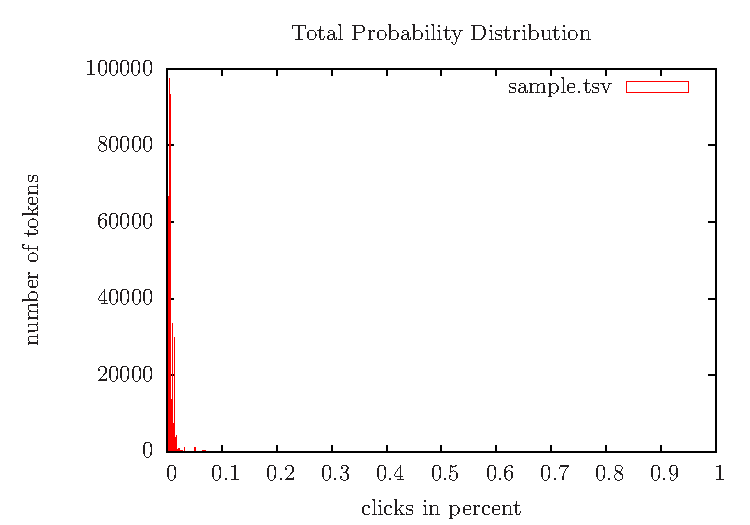
\includegraphics[width=8cm]{scriptplot.pdf}
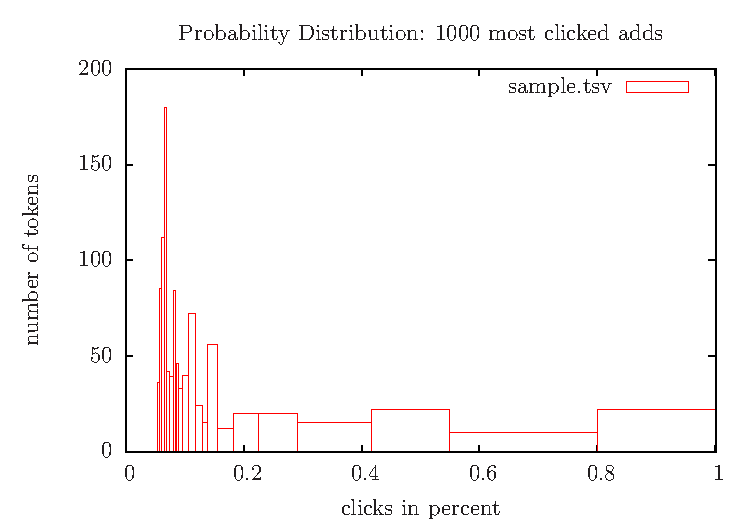
\includegraphics[width=8cm]{scriptplot3.pdf}
}
      \caption{
		Histogram of the probabilities found for the whole set studied on the left. 
		On the right, the same plot but considering the $1000$ most clicked items only.
		The most clicked adds have
		an astonishing statistics as their counts is quite constant.
		This is either due to statistical anomalies or very efficient adds. 
		$22$ adds have made a perfect score.	
              }
\label{thxalbert}
\end{figure}




\end{document}

